% 2016 全国卷Ⅰ理科第 7 题：函数图象选择项 A–D。
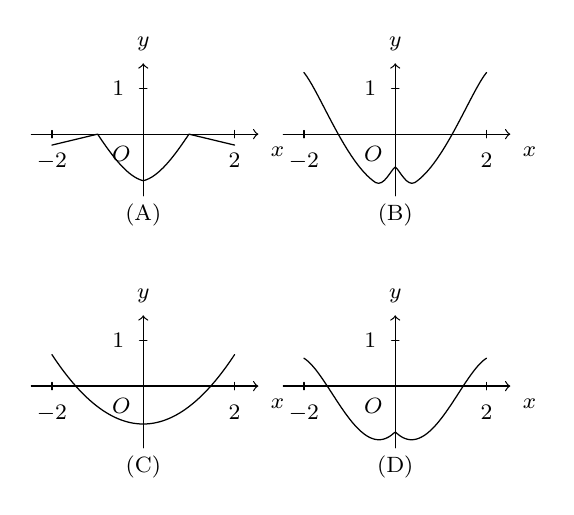
\begin{tikzpicture}[x=.58cm,y=.58cm,font=\footnotesize,line width=.45pt,
  line cap=round,line join=round]
  % A：两侧在 x 轴下方，曲线在 x=±1 处到达尖点。
  \begin{scope}[yshift=3.2cm]
    \draw[->] (-2.45,0) -- (2.52,0);
    \draw[->] (0,-1.35) -- (0,1.55);
    \draw (-2,.08)--(-2,-.08) node[below=2pt] {$-2$};
    \draw (2,.08)--(2,-.08) node[below=2pt] {$2$};
    \draw (.08,1)--(-.08,1) node[left=2pt] {$1$};
    \node[below left=1pt] at (0,0) {$O$};
    \node[below right=1pt] at (2.52,0) {$x$};
    \node[above=1pt] at (0,1.55) {$y$};
    \draw (-2,-.24) -- (-1,0)
      .. controls (-.68,-.48) and (-.34,-.94) .. (0,-1.02)
      .. controls (.34,-.94) and (.68,-.48) .. (1,0)
      -- (2,-.24);
    \node at (0,-1.76) {(A)};
  \end{scope}

  % B：两端高于 y=1，中央为带尖顶的双谷。
  \begin{scope}[xshift=3.2cm,yshift=3.2cm]
    \draw[->] (-2.45,0) -- (2.52,0);
    \draw[->] (0,-1.35) -- (0,1.55);
    \draw (-2,.08)--(-2,-.08) node[below=2pt] {$-2$};
    \draw (2,.08)--(2,-.08) node[below=2pt] {$2$};
    \draw (.08,1)--(-.08,1) node[left=2pt] {$1$};
    \node[below left=1pt] at (0,0) {$O$};
    \node[below right=1pt] at (2.52,0) {$x$};
    \node[above=1pt] at (0,1.55) {$y$};
    \draw (-2,1.35)
      .. controls (-1.65,.92) and (-1.08,-.63) .. (-.43,-1.06)
      .. controls (-.25,-1.16) and (-.10,-.79) .. (0,-.72)
      .. controls (.10,-.79) and (.25,-1.16) .. (.43,-1.06)
      .. controls (1.08,-.63) and (1.65,.92) .. (2,1.35);
    \node at (0,-1.76) {(B)};
  \end{scope}

  % C：两端高于 x 轴，中央为平滑单谷。
  \begin{scope}
    \draw[->] (-2.45,0) -- (2.52,0);
    \draw[->] (0,-1.35) -- (0,1.55);
    \draw (-2,.08)--(-2,-.08) node[below=2pt] {$-2$};
    \draw (2,.08)--(2,-.08) node[below=2pt] {$2$};
    \draw (.08,1)--(-.08,1) node[left=2pt] {$1$};
    \node[below left=1pt] at (0,0) {$O$};
    \node[below right=1pt] at (2.52,0) {$x$};
    \node[above=1pt] at (0,1.55) {$y$};
    \draw[domain=-2:2,samples=80,variable=\x]
      plot ({\x},{.38*\x*\x-.83});
    \node at (0,-1.76) {(C)};
  \end{scope}

  % D：按题给函数绘出对称双谷，端点位于 x 轴上方、y=1 下方。
  \begin{scope}[xshift=3.2cm]
    \draw[->] (-2.45,0) -- (2.52,0);
    \draw[->] (0,-1.35) -- (0,1.55);
    \draw (-2,.08)--(-2,-.08) node[below=2pt] {$-2$};
    \draw (2,.08)--(2,-.08) node[below=2pt] {$2$};
    \draw (.08,1)--(-.08,1) node[left=2pt] {$1$};
    \node[below left=1pt] at (0,0) {$O$};
    \node[below right=1pt] at (2.52,0) {$x$};
    \node[above=1pt] at (0,1.55) {$y$};
    \draw[domain=-2:2,samples=120,variable=\x]
      plot ({\x},{2*\x*\x-exp(abs(\x))});
    \node at (0,-1.76) {(D)};
  \end{scope}
\end{tikzpicture}
